\chapter{Deep Learning}

\section{Was ist Deep Learning?}

Unter \textbf{Deep Learning} (zu deutsch tiefes Lernen) versteht man ein Teilgebiet des maschinellen Lernens, welches sich mit künstlichen neuronalen Netzen und große Datenmengen befasst. Es eignet sich für eine Vielzahl von Anwendungsfällen wie beispielsweise für selbstfahrende Autos, in der Medizin als auch im Marketing. \cite{datasolut2}\\

Mit Deep Learning können Probleme gelöst werden, die ohne diese Ansätze nicht lösbar wären. Tiefes Lernen ist allerdings sehr rechenaufwändig, wodurch das Training über Monate hinweg andauern kann, um gute Entscheidungen treffen zu können. Gründe hierfür sind komplexe Architekturen sowie eine Vielzahl an Modell-Parametern. \cite{datasolut2} \\

\begin{figure}[H]
	\centering
	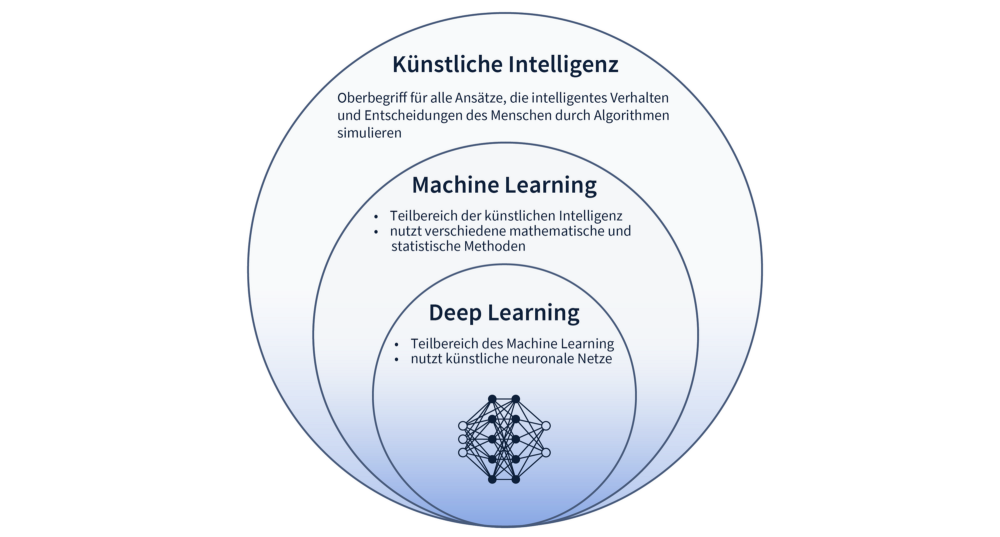
\includegraphics[width=\textwidth]{kapitel3/images/KI_Uebersicht.png}
	\caption{Übersicht Künstliche Intelligenz}
	\vspace{0.2cm}
	\quelle\url{https://datasolut.com/wp-content/uploads/2019/11/KI-und-Deep-Learning.002-e1558385989498.jpeg}
\end{figure}

Die Grundlage des Deep Learnings stellt die Verwendung von künstlichen neuronalen Netzen dar. Unter künstlichen neuronalen Netzen versteht man Algorithmen, die nach dem biologischen Vorbild des menschlichen Gehirns modelliert sind. Diese werden eingesetzt, um beispielsweise Muster in Bildern zu erkennen oder Bilder zu klassifizieren. \cite{datasolut2}\\

\newpage

Ein einfaches künstliches neuronales Netz besteht dabei aus einer \textbf{Eingabeschicht} (Input Layer), einer \textbf{Zwischenschicht} (Hidden Layer) und einer \textbf{Ausgabeschicht} (Output Layer). \cite{datasolut2}

\begin{figure}[H]
	\centering
	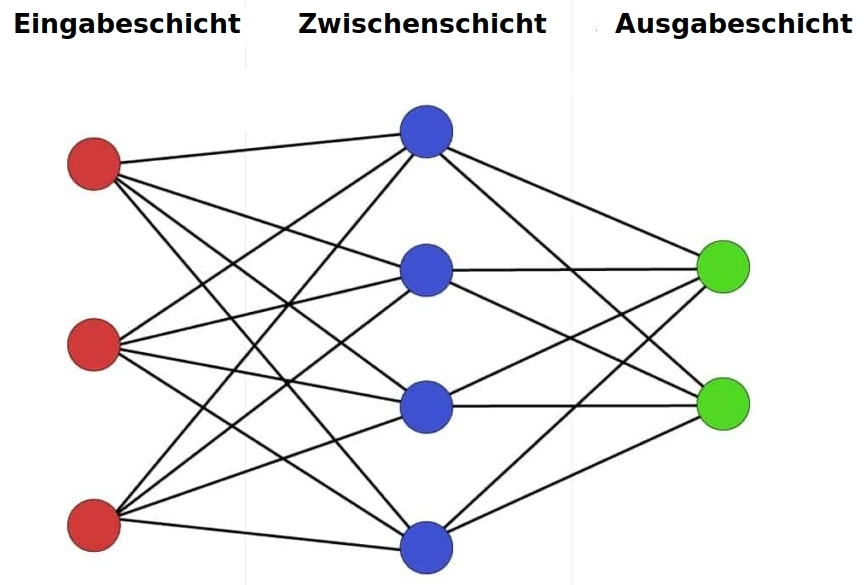
\includegraphics[width=0.65\textwidth]{kapitel3/images/Simples_Neuronales_Netz.jpg}
	\caption{Darstellung eines beispielhaften künstlichen neuronalen Netzes \\ (vereinfacht)}
	\label{fig:simples-neuronales-netz}
	\vspace{0.2cm}
	\quelle\url{https://datasolut.com/wp-content/uploads/2019/10/ku%CC%88nstliche-neuronale-Netze.jpg}
\end{figure}

Von tiefem Lernen spricht man dann, wenn die eingesetzten neuronalen Netze mehr als eine Zwischenschicht haben.  \cite{datasolut2} 

\section{Warum Deep Learning?}

Es gibt Problemstellungen (wie beispielsweise die unstrukturierte Bilderkennung), die sich besonders gut mit künstlichen neuronalen Netzen lösen lassen. Das Erlernen dieser komplexen Muster ist jedoch mit klassischen Machine Learning Algorithmen nur sehr schwer lösbar. Hier kommen dann tiefe künstliche neuronale Netze zum Einsatz. Je größer die Datenmenge ist, die zum lernen verwendet wird, desto besser funktioniert das tiefe Lernen. \cite{datasolut2}

\begin{figure}[H]
	\centering
	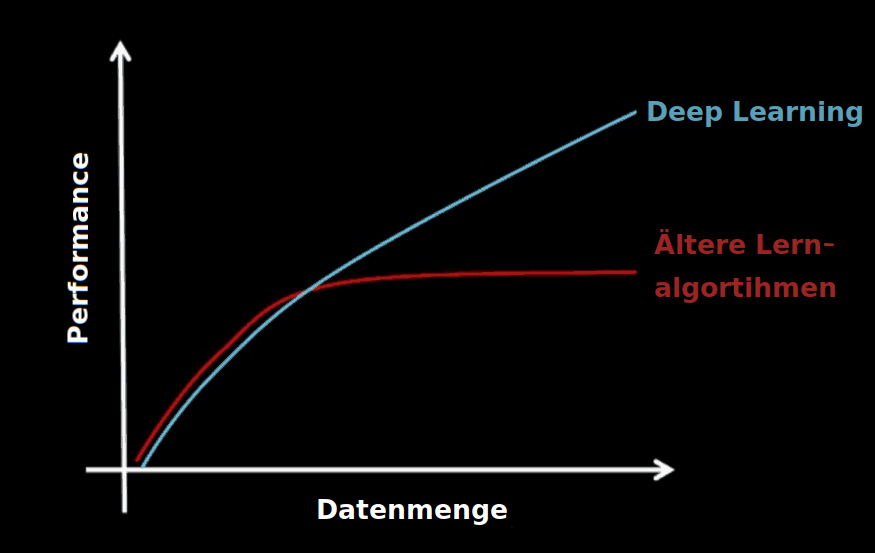
\includegraphics[scale=0.4]{kapitel3/images/Deep_Learning_Performance.png}
	\label{fig:deep-learning-performance}
	\caption{Darstellung der Performance von Deep Learning Algorithmen im Vergleich zu älteren Lernalgorithmen}
	\vspace{0.2cm}
	\quelle\url{https://datasolut.com/wp-content/uploads/2019/11/Warum-deep-learning-1024x742.png}
\end{figure}

\section{Lernverfahren}

Beim maschinellen Lernen bzw. beim Deep Learning stehen drei unterschiedliche \textbf{Lernverfahren} zur Verfügung:

\subsection{Überwachtes Lernen (Supervised Learning)}

	Das \textbf{überwachte Lernen} nutzt für den Lernprozess \textbf{bekannte Daten}, um daraus Muster und Zusammenhänge zu erkennen. Die Muster werden  anhand eines \textbf{Trainingsdatensatzes} (Beispieldaten) erlernt. Dabei wird der Zusammenhang zu einer Zielvariable erlernt und es wird versucht diese richtig vorherzusagen. \cite{datasolut3}

\subsection{Unüberwachtes Lernen (Unsupervised Learning)}

	Das \textbf{unüberwachte Lernen} nutzt für den Lernprozess keine Beispieldaten, sondern \textbf{Rohdaten}, aus denen eigenständig Muster erkannt werden sollen. \\
	Der hauptsächliche Unterschied zum überwachten Lernen ist also, dass das unüberwachte Lernen nicht dafür ausgelegt ist, eine Vorhersage für eine bekannte Zielvariable zu treffen. \cite{datasolut3}
	
\subsection{Bestärkendes Lernen (Reinforcment Learning)}

	Anders als das überwachte bzw. unüberwachte Lernen nutzt das \textbf{bestärkende Lernen} zunächst \textbf{keine Daten}, sondern diese entstehen in einer Simulationsumgebung nach einem \textbf{Versuch-und-Irrtum-Verfahren}. \cite{der-onliner_blogspot}
	
\begin{figure}[H]
	\centering
	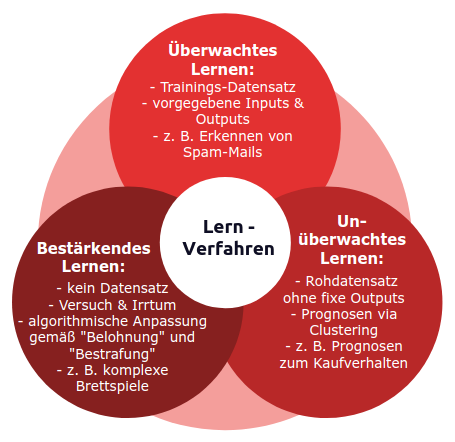
\includegraphics[width=0.6\textwidth]{kapitel3/images/lernverfahren.png}
	\label{fig:machine-learning-algorithms}
	\caption{Darstellung der verschiedenen Lernverfahren}
	\vspace{0.2cm}
	\quelle\url{https://1.bp.blogspot.com/-xstYqLb9OBw/XSYZUUD0WrI/AAAAAAAAML4/4sxvpGjIsDgmR7bDYyhcKdfM0TbvIIHdwCEwYBhgL/s400/machine-learning-lernverfahren.png}
\end{figure}

Welches Lernverfahren schlussendlich eingesetzt wird, hängt hierbei vom Anwendungsfall ab sowie mit den daraus resultierenden Datensätzen.

\section{Datensatz}

Damit ein künstliches neuronales Netz mit überwachtem Lernen, seine Aufgabe erfüllen kann, muss zunächst ein \textbf{Datensatz} erstellt werden, damit das Netz trainiert werden kann. Der Datensatz besteht dabei aus einem \textbf{Trainingsdatensatz}, einem \textbf{Validierungsdatensatz} sowie aus einem \textbf{Testdatensatz}. \\

\subsection{Trainingsdatensatz}

Der \textbf{Trainingsdatensatz} ist ein Beispieldatensatz der für das \textbf{Lernen} der Muster und Zusammenhänge in den Daten verwendet wird. Das Modell des neuronalen Netz nutzt also diese Daten um zu lernen. \cite{datasolut} \\

\subsection{Validierungsdatensatz}

Der \textbf{Validierungsdatensatz} ist ebenso ein Beispieldatensatz, welcher für die \textbf{Abstimmung der Hyperparameter} des Modells des neuronalen Netzes verwendet wird. Dadurch wird das sogenannte \glqq Overfitting\grqq{} (Überanpassung) des Modells auf die Trainingsdaten verhindert. \cite{datasolut} \\

\subsection{Testdatensatz}

Der \textbf{Testdatensatz} ist ebenfalls ein Beispieldatensatz, jedoch sind die Daten von den Trainingsdaten unabhängig. Die Testdaten werden beim Training des neuronalen Netzes nicht benutzt, sondern dienen zur abschließenden \textbf{Verifikation} des Modells. Dadurch kann die Qualität des Modell erfasst werden, damit man eine Aussage über die Leistungsfähigkeit des neuronalen Netzes treffen kann. \cite{datasolut} \\

\section{Funktionsweise und Aufbau künstlicher neuronaler Netze}

Die \textbf{Neuronen} (Knotenpunkte) eines künstlichen neuronalen Netzes sind \textbf{schichtweise} angeordnet. Diese werden normalerweise in einer festen Hierarchie miteinander verbunden. Die Neuronen sind dabei im Regelfall zwischen zwei Schichten verbunden, jedoch in Ausnahmefällen aber auch innerhalb einer Schicht. \cite{jaai} \\

Die Informationen fließen beginnend mit der Eingabeschicht über eine oder mehrere Zwischenschichten bis hin zur Ausgabeschicht. Dabei ist der Ausgabewert eines Neurons der Eingabewert des nächsten Neurons. \cite{jaai} \\

Künstliche neuronale Netze werden meist schematisch horizontal dargestellt (wie z.B. in Abbildung \ref{fig:simples-neuronales-netz}). Die Eingabeschicht befindet sich dabei auf der linken Seite  gefolgt von den Zwischenschichten in der Mitte und der Ausgabeschicht auf der rechten Seite.
Die Anzahl der Schichten die in einem künstlichen neuronalen Netz verwendet werden, ist eine wichtige beschreibende Information. Enthält ein Netz zum Beispiel drei Schichten, so spricht man von einem drei-schichtigen neuronalen Netz. \cite{jaai}

\subsection{Eingabeschicht (input layer)}
	
	Die \textbf{Eingabeschicht} definiert den \textbf{Startpunkt} des Informationsflusses in einem künstlichen neuronalen Netz. Die Eingangssignale werden dabei von den Neuronen am Anfang dieser Schicht entgegengenommen und am Ende gewichtet an die Neuronen der ersten Zwischenschicht weitergegeben. \cite{jaai}
	
\subsection{Zwischenschichten (hidden layer)}

	\textbf{Zwischen} der Eingabe- und der Ausgabeschicht befindet sich mindestens eine \textbf{Zwischenschicht}. Je \textbf{mehr} Zwischenschichten ein künstliches neuronales Netz besitzt, desto \textbf{tiefer} ist das Netz, jedoch bewirkt jede weitere hinzukommende Zwischenschicht auch einen Anstieg der benötigten Rechenleistung. \cite{jaai}
	
\subsection{Ausgabeschicht (output layer)}

	Die \textbf{Ausgabeschicht} bildet die \textbf{letzte} Schicht eines künstlichen neuronalen Netzes, wobei diese sich hinter den Zwischenschichten befindet. Sie stellt das \textbf{Ende} des Informationsflusses eines künstlichen neuronalen Netz dar und enthält das \textbf{Ergebnis} der Informationsverarbeitung. \cite{jaai}
	
\subsection{Modellparameter}

Die \textbf{Modellparameter} eines künstlichen neuronalen Netzes werden beim Training des Netzes \textbf{selbständig} erlernt. Basierend auf bereits vorhandenen Parametern trainiert der Trainingsalgorithmus und versucht dadurch, die Modellparameter immer weiter zu verbessern. \cite{divis}

\subsection{Hyperparameter}

Die \textbf{Hyperparameter} eines künstlichen neuronalen Netz dienen zur Steuerung des Trainingsalgorithmus. In der Regel müssen die Werte der Hyperparameter im Gegensatz zu den Modellparametern \textbf{vor} dem eigentlichen Training des Modells festgelegt werden, wodurch diese \textbf{nicht selbständig} erlernt werden können. \cite{wiki} \\

Einige Beispiele für Hyperparameter sind:

\begin{enumerate}
	\item \textbf{Lerngeschwindigkeit} (learning rate)
	\item \textbf{Batch Size}
	\item \textbf{Anzahl Epochen}
	\item \textbf{Optimizer}
	\item \textbf{Dropout}
\end{enumerate}
	
\subsection{Gewichte und Verzerrung (Bias)}

	Durch die \textbf{Gewichte} wird die \textbf{Intensität} des Informationsflusses entlang einer Verbindung eines künstlichen neuronalen Netzes beschrieben. Dazu vergibt jedes Neuron ein Gewicht für die durchfließende Information. Diese wird anschließend mit diesem Gewicht gewichtet und es wird ein Wert für die neuronen-spezifische \textbf{Verzerrung} (Bias) addiert. Das resultierende Ergebnis wird in der Regel durch eine sogenannte \textbf{Aktivierungsfunktion} geleitet, bevor es an die Neuronen der nächsten Schicht weitergegeben wird. \cite{jaai} \\
	
	Während des Trainingsprozesses werden die Gewichte und Verzerrungen so angepasst, dass das Endresultat möglichst \textbf{genau} den Anforderungen entspricht. \cite{jaai}
	
\subsection{Aktivierungsfunktion (activation function)}

	\textbf{Aktivierungsfunktionen} spielen in künstlichen neuronalen Netzen eine bedeutende Rolle, da sie dabei helfen, die \textbf{komplizierte} und \textbf{nichtlineare funktionale Beziehung} zwischen den \textbf{Eingangsdaten} und den abhängigen \textbf{Ergebnissen} zu lernen und zu verstehen. Ein Eingangssignal eines Neurons wird dabei in ein Ausgangssignal konvertiert, welches anschließend als Eingabe der nächsten Schicht verwendet wird. \cite{ai-united} \\
	
	Einige Beispiele für Aktivierungsfunktionen sind:
	
	\begin{center}
	\begin{tabular}[t]{|c|c|c|}
		\hline
		\textbf{Bezeichnung} & \textbf{Funktion} & \textbf{Plot} \\
		\hline
		\begin{tabular}{l} Identität \end{tabular} &  
		\begin{tabular}{l} $ f(x) = x $ \end{tabular} &
		\begin{tabular}{l}
			\addvbuffer[0.05cm]{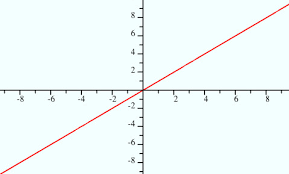
\includegraphics[scale=0.5]{kapitel3/images/idendity.png}}
		\end{tabular} \\
		\hline
		\begin{tabular}{l} Sigmoid \end{tabular} &  
		\begin{tabular}{l} $ f(x) = \frac{1}{1 + e^{-x}} $ \end{tabular} &
		\begin{tabular}{l}
			\addvbuffer[0.05cm]{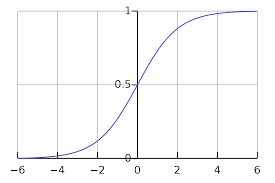
\includegraphics[scale=0.5]{kapitel3/images/sigmoid.png}}
		\end{tabular} \\
		\hline
		\begin{tabular}{l} ReLu \end{tabular} &  
		\begin{tabular}{l} $ f(x) = \max (0,x) $ \end{tabular} &
		\begin{tabular}{l}
			\addvbuffer[0.05cm]{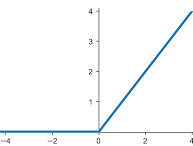
\includegraphics[scale=0.5]{kapitel3/images/relu.png}}
		\end{tabular} \\
		\hline
	\end{tabular}
	\end{center}

	\begin{center}
	\begin{tabular}[t]{|c|c|c|}
		\hline
		\textbf{Bezeichnung} & \textbf{Funktion} & \textbf{Plot} \\
		\hline
		\begin{tabular}{l} ELu \end{tabular} &  
		\begin{tabular}{l} $ f(\alpha, x) = \begin{cases} \alpha (e^x - 1) \quad \textrm{für} \ x \leq 0 \\ x \hspace{1.75cm} \textrm{für} \ x > 0 \end{cases} $ \end{tabular} &
		\begin{tabular}{l}
			\addvbuffer[0.05cm]{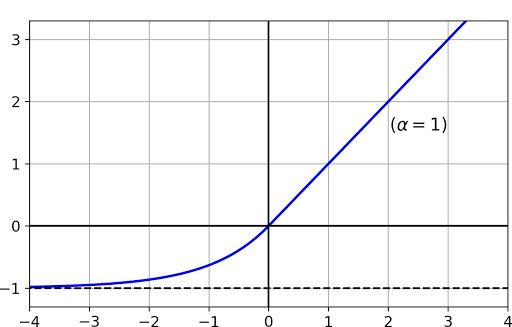
\includegraphics[scale=0.25]{kapitel3/images/elu.jpg}}
		\end{tabular} \\
		\hline
	\end{tabular}
	\end{center}

\subsection{Verlustfunktion (loss function)}

	Die \textbf{Verlustfunktion} wird zur \textbf{Berechnung des Fehlers} zwischen den realen Ergebnissen und erhaltenen Antworten des künstlichen neuronalen Netzes verwendet. Das Ziel des Lernprozesses ist die \textbf{Minimierung} dieser Fehler.  \cite{ai-united} \\

	Einige Beispiele für Verlustfunktionen sind:
	
	\begin{center}
	\begin{tabular}[t]{|l|l|}
		\hline
		\textbf{Bezeichnung} & \textbf{Funktion} \\
		\hline
		Mittlere quadratische Abweichung  &  
		\addvbuffer[0.05cm]{
			$ \textrm{MSE} = \frac{\sum_{i=1}^{n} (y_i - \hat{y_i})^2}{n} $
		} \\
		\hline
		Mittlerer absoluter Fehler  &  
		\addvbuffer[0.05cm]{
			$ \textrm{MAE} = \frac{\sum_{i=1}^{n} |y_i - \hat{y_i}|}{n} $
		} \\
		\hline
		Mittlerer Bias Fehler  &  
		\addvbuffer[0.05cm]{
			$ \textrm{MBE} = \frac{\sum_{i=1}^{n} (y_i - \hat{y_i})}{n} $
		} \\
		\hline
		
	\end{tabular}
	\end{center}

\subsection{Fehlerrückführung (Backpropagation)}

	Bei der \textbf{Fehlerrückführung} wird die Antwort des künstlichen neuronalen Netzes mit dem gewünschten Ergebnis verglichen. Dabei wird der Fehler bestimmt und dieser wird anschließend \textbf{rückwärtig} in das Netz gespeist, wodurch die Gewichte der Neuronen so angepasst werden, dass der Fehler immer \textbf{kleiner} wird. In der Praxis werden dafür verschiedene \textbf{Optimierungsstrategien} eingesetzt. \cite{rocketloop}
	
\subsubsection{Optimierungsstrategien (Optimizer)}

	\begin{enumerate}
		\item \textbf{Gradientenverfahren:}
		
			Das Gradientenverfahren beschreibt einen Algorithmus, der für eine Verlustfunktion, den Eingabeparameter in entgegengesetzter Richtung des Gradienten aktualisiert. Über die  Lerngeschwindigkeit (learn rate) kann festgelegt werden, wie weit der Algorithmus sich in jeder Iteration vom Ausgangspunkt entfernen darf. \cite{lucas_plagwitz}
		
		\item \textbf{Momentum Optimierer:}
		
			Der Momentum Optimierer ist ein erweiterter Ansatz des Gradientenverfahrens. Während das \glqq Standardgradientenverfahren\grqq{} in jedem Iterationsschritt immer in entgegengesetzte Richtung des lokalen Gradienten absteigt, nimmt der Momentum Optimierer Rücksicht auf die Gradienten der vorherigen Iterationen. \cite{lucas_plagwitz}
			
		\item \textbf{Adaptive Optimierungsstrategie:}
		
			Ein Abstiegt wie ihn die Gradientenverfahren erledigen, kann unter Umständen nicht dir richtige Wahl zur Lösung des Problems darstellen. Daher wurden adaptive Algorithmen entwickelt, die eine Alternative zu den Gradientenverfahren darstellen. Dabei wird folgende Idee verfolgt: Man passt die Lernrate dynamisch an die Parameter an und führt größere Aktualisierungen für seltene Parameter durch und kleinere Aktualisierungen für häufige Parameter. \cite{lucas_plagwitz}
			
			\begin{enumerate}
				\item \textbf{AdaGrad:}
				
					Der Kerngedanke hinter AdaGrad ist das Herunterskalieren des Gradientenvektors, d.h. die Lernrate wird pro Dimension nach und nach verringert, wobei die Verringerung bei steilen Dimensionen schneller erfolgt. \cite{lucas_plagwitz}
					
				\item \textbf{RMSProp:}
				
					RMSProp ist eine leicht modifizierte Version des AdaGrad Optimierers. Dabei werden die Gradienten der letzten Iterationen unter exponentiellem Zerfall  berücksichtigt. Im Allgemeinen lässt sich sagen, dass RMSProp schneller konvergiert als AdaGrad. \cite{lucas_plagwitz}
				
					
			\end{enumerate}
		
			
		\item \textbf{Adam Optimierung:}
		
			Die Adam Optimierung ist eine Kombination aus der Idee des Momentum Optimierers und RMSProp. Das Verfahren betrachtet hierbei sowohl den Durchschnitt der vorigen Gradienten als auch den Durchschnitt der quadrieten Gradienten, beide unter exponentiellem Zerfall. \cite{lucas_plagwitz}
			
	\end{enumerate}

\section{Arten von  künstlichen neuronalen Netzen}

Es gibt eine Vielzahl von künstlichen neuronalen Netzwerk-Architekturen. Im folgenden wird auf die wichtigsten Arten eingegangen:

\subsection{Perceptron}

	Ein \textbf{Perceptron} ist das einfachste künstliche neuronale Netz. Es nimmt die Eingabeparameter entgegen, addiert diese, wendet die Aktivierungsfunktion an und schickt das Ergebnis an die Ausgabeschicht. Das Ergebnis ist hierbei binär und somit vergleichbar mit einer Ja- bzw. Nein-Entscheidung. Die Entscheidung erfolgt dadurch, dass der Wert der Aktivierungsfunktion mit einem Schwellwert verglichen wird. Wird der Schwellwert unterschritten, so wird dem Ergebnis 0 zugeordnet und bei einer Überschreitung des Schwellwerts wird dem Ergebnis 1 zugeordnet.
	
	\begin{figure}[H]
		\centering
		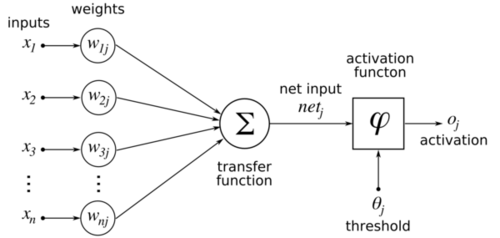
\includegraphics[width=0.8\textwidth]{kapitel3/images/perceptron.png}
		\caption{Darstellung eines Perceptrons}
		\vspace{0.2cm}
		\quelle\url{https://upload.wikimedia.org/wikipedia/commons/thumb/f/ff/Rosenblattperceptron.png/500px-Rosenblattperceptron.png}
		\end{figure}

\subsection{Fully Connected Neural Networks (FCNNs)}

	\textbf{Fully Connected Neural Networks} (FCNNs) zeichnen sich dadurch aus, dass die Schichten immer nur mit der nächst höheren Schicht verbunden sind, d.h. es gibt \textbf{keine} zurückgerichteten Kanten. \cite{datasolut4}
	
	\begin{figure}[H]
		\centering
		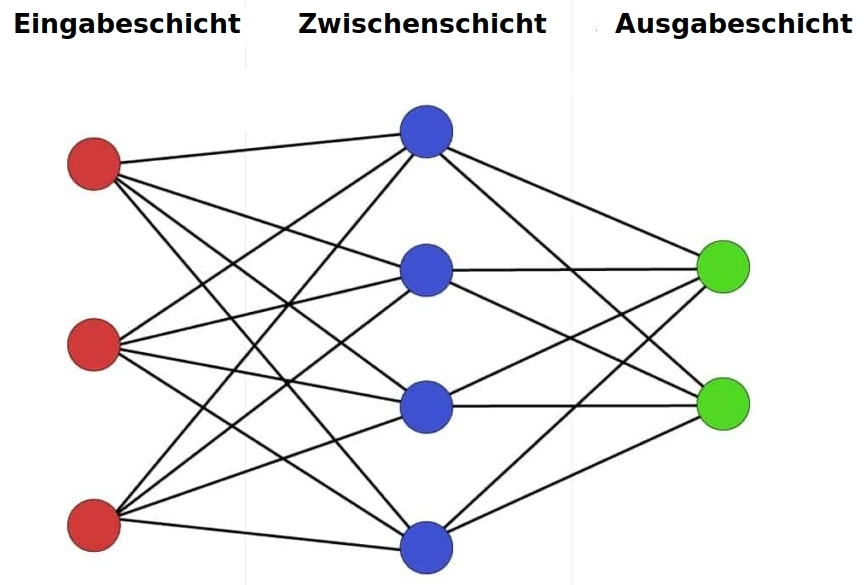
\includegraphics[width=0.65\textwidth]{kapitel3/images/Simples_Neuronales_Netz.jpg}
		\caption{Darstellung eines beispielhaften FCNN}
		\vspace{0.2cm}
		\quelle\url{https://datasolut.com/wp-content/uploads/2019/10/ku%CC%88nstliche-neuronale-Netze.jpg}
	\end{figure}

\subsection{Convolutional Neural Networks (CNNs)}

	\textbf{Convolutional Neural Networks} (CNNs) können besonders effizient mit 2D- bzw. 3D-Eingabedaten arbeiten. Insbesondere werden CNNs für die Objektdetektion in Bildern angewendet. \cite{datasolut4} \\
	
	\begin{figure}[H]
		\centering
		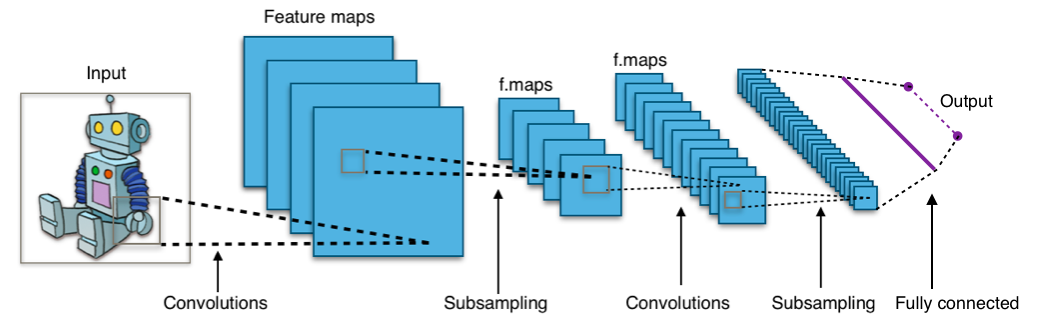
\includegraphics[width=0.9\textwidth]{kapitel3/images/cnn.png}
		\caption{Darstellung eines beispielhaften CNN}
		\vspace{0.2cm}
		\quelle\url{https://de.wikipedia.org/wiki/Convolutional_Neural_Network#/media/Datei:Typical_cnn.png}
	\end{figure}
	
	Der Unterschied zu den klassischen künstlichen neuronalen Netzen liegt in der Architektur der CNNs: Die Zwischenschicht basiert hierbei auf einer Abfolge von Faltungs- und Poolingoperationen. Bei der Faltung wird ein sogenannter Faltungskernel über die Daten geschoben und das Ergebnis der Faltungsoperation wird berechnet. Anschließend werden die Neuronen aktualisiert. Die nachfolgende Poolingoperation sorgt dann dafür, dass die Ergebnisse vereinfacht werden. Dadurch bleiben nur die wichtigsten Informationen erhalten.	Des Weiteren wird dadurch erreicht, dass die 2D- oder 3D-Eingangsdaten kleiner werden. \cite{datasolut4} 

\subsection{Recurrent Neural Networks (RNNs)}

	Bei den \textbf{Recurrent Neural Networks} (RNNs) werden der Netzstruktur wiederkehrende Zellen hinzugefügt, wodurch das Netz eine Art  Gedächtnis erhält. \cite{datasolut4} \\ 
	
	\begin{figure}[H]
		\centering
		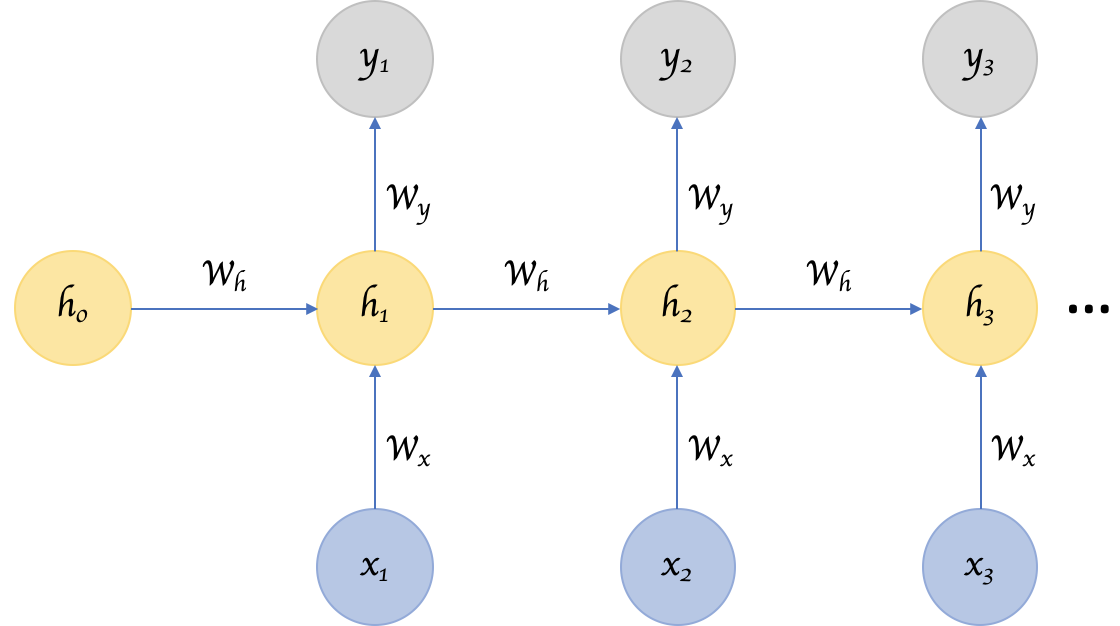
\includegraphics[width=0.9\textwidth]{kapitel3/images/rnn.png}
		\caption{Darstellung eines beispielhaften RNN}
		\vspace{0.2cm}
		\quelle\url{https://datasolut.com/wp-content/uploads/2020/09/recurrent-neuronal-network.png}
	\end{figure}
	
	
	RNNs werden insbesondere dann eingesetzt, wenn der Kontext wichtig ist. Dadurch beeinflussen Entscheidungen aus vergangenen Iterationen maßgeblich die aktuellen Entscheidungen. \cite{datasolut4} \\
	
	Recurrent Neural Networks besitzen jedoch einen entscheidenden Nachteil: Sie werden über die Zeit instabil. Um dies zu verhindern werden sogenannte Long Short-Term Memory Units (LSTMs) eingesetzt. Diese stabilisieren Netz auch für Abhängigkeiten, die über einen längeren Zeitraum bestehen. \cite{datasolut4}





